%!TEX root = ../../main.tex
\subsection{Smart Contracts}
\label{ch:approach:intro:smartcontracts}

There is one specific technology created by the Ethereum Foundation which allowed for the first time the embedding of source code into the Blockchain called \emph{smart contract}.

A smart contract is a piece of structured code embedded into the Blockchain; it uses an \ac{API} to interact with the chain. Once in a block, it cannot be altered, but new versions and improvements can be reinserted. There is an implicit economical cost for submitting intelligent contracts into the chain and executing functions that will generate new blocks. Anyone willing to participate and be part of the contract must be a member of a \ac{DAO} or \ac{DAC}, use a public and key as a unique identity and a private key to sign the transaction being submitted. Generally speaking, smart contracts are public and can be easily visualized to know the conditions and rules that the involved parties will use to interact. Ethereum Network was the first blockchain to implement the generation and execution of Smart Contracts fully. 

In the white paper \cite{Ethereum30:online}, it stipulates the basis for the usage of \emph{Custom currencies} ans \emph{colored coins} (first integrated in the Bitcoin Blockchain) and how they can be extended to the usage of custom tokens coded in a \emph{Turing Complete}\footnote{A concept named after English mathematician and computer scientist Alan Turing- a system of data-manipulation rules (such as a computer's instruction set, a programming language, or a cellular automaton) is said to be "Turing complete" or "computationally universal" if it can be used to simulate any Turing machine.} programming language.

Smart Contracts have proved to be flexible and adaptable to deploy applications where trust and decentralization is vital. The technology is relatively new. Since 2015 many organizations have joined forces to include new programming language in different sets of ledgers. For the \emph{Ethereum} Blockchain the standard language is known as \emph{Solidity}\cite{SolidityEthereum:online}. With the arrival of other Systems, new programming languages where created whereas others like the  \emph{Hyperledger Foundation} implement \emph{JavaScript}, \emph{Java}, \emph{Go} and \emph{Solidity as well}.

They also allowed the creation of \ac{DAO}s, where multiple parties could cooperate and collaborate in the benefit of the Blockchain ecosystem by agreeing on the rules that the smart contract was intended to execute depending on the conditions and situations the users will perform as a result of interacting with the \ac{DLT}.

This phenomenon called the attention of the industry for its potential to cooperate and create immutable database systems, but adapted to an anonymous and permissioned approach.

\subsubsection{Non-fungibility}
\ac{NFT}\footnote{An object is fungible when and if it is identical to others and thus can be replaced without any loss (mutual interchangeability). On the other hand, an object is non-fungible if it posses unique properties, making it unequal to others and thus of a different transactional value than their reciprocals.} in the blockchain brings tremendous possibilities to store value and a representation of physical or virtual objects. When the concept was exploited and implemented for the first time as a true standard in the Ethereum Environment\cite{EIP721No48:online}, \footnote{Ethereum is another decentralized open source blockchain with smart contract functionality embedded since its conception. Conceived in 2013, its creator extended the potential that Bitcoin had as a decentralized system to enable the generation of digital contracts.} the public realized of the potential the technology could have to generate value over the issuance of public certificates able to be verified by anyone to proof authenticity or ownership for predefined assets. 

Although \ac{NFT}s have skyrocketed from public Blockchains to demonstrate their potential with digital art (paintings, music, certification of authenticity, among others), little has been researched and implemented in the industry. But Non-fungibility has proven to be a key player for future technologies and mutual collaboration. Having a system with which companies can implicitly trust and collaborate offers tremendous possibilities for the development of knowledge and data protection.

\begin{figure}[h]
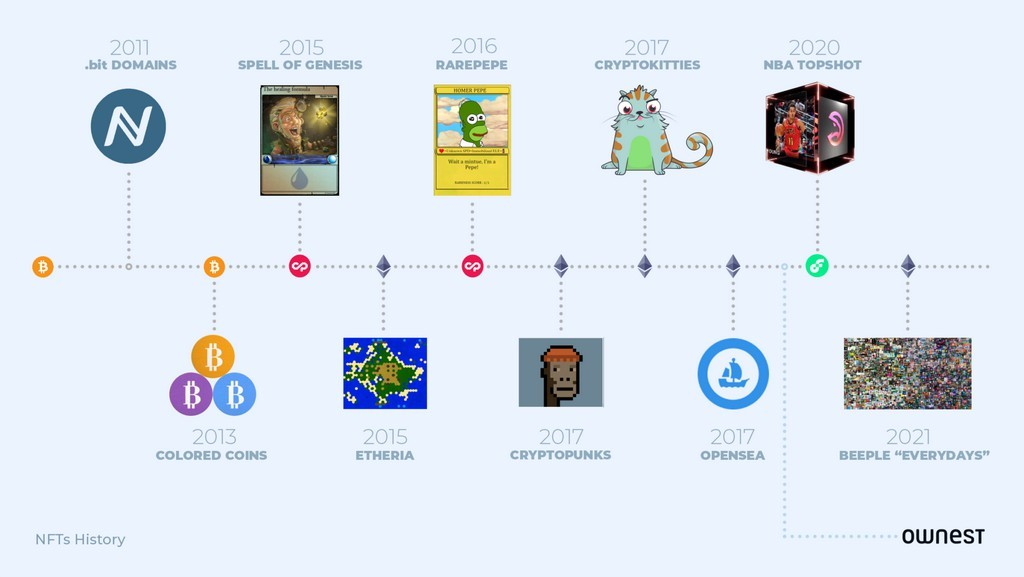
\includegraphics[width=15cm]{img/01-NFT_Timeline.png}
\centering
\caption{NFT Timeline, from the creation of Bitcoin domains, coloured coins to the new Ethereum and Altcoin derivatives  \cite{OwnestNF21:online}}
\end{figure}

Industries can nowadays benefit from blockchain systems to record and track data in more trustful ways and allow inter-entity cooperation. However, the problem of privacy, ownership, security and finance emerges when trying to implement such systems on a public blockchain. 
